%----------------------------------------------------------------------------------------
%   PACKAGES AND THEMES
%----------------------------------------------------------------------------------------

\documentclass{beamer}

\mode<presentation> {
\usetheme{Madrid}
\usecolortheme{crane}
}
\usepackage{listings}
\usepackage{graphicx} 
\usepackage{booktabs} 
\usepackage[italian]{babel}
\usepackage[utf8]{inputenc}
\usepackage[T1]{fontenc}
\usepackage{setspace}
\usepackage{listing}

%----------------------------------------------------------------------------------------
%   TITLE PAGE
%----------------------------------------------------------------------------------------

\title[Seminario ATPL 17/18]{Lambda Expressions in Java 8: Uso e Tipaggio} 
\author[]{Mattia D'Autilia - 5765968 - mattia.dautilia@stud.unifi.it,\\ Alex Foglia - 6336805 - alex.foglia@stud.unifi.it}
\date{}

\begin{document}

%------------------------------------------------

\begin{frame}
	\frametitle{\textbf{Presentazione Seminario ATPL : 2017/2018}}
	\begin{center}
  		
\includegraphics[width=0.2\textwidth]{assets/logo-unifi.png}
  	\end{center}
	\titlepage 
\end{frame}

%------------------------------------------------

\begin{frame}
	\frametitle{\textbf{Indice presentazione}}
	\begin{large}
	\begin{enumerate}
		\item
			\textbf{Java e Java 8}\\\
		\item
			\textbf{Lambda Expression in Java 8}\\\
		\item
			\textbf{Tipaggio Lambda Expression}\\\
		\item
			\textbf{Lambda Expression vs Design Pattern}\\\
		\item			
			\textbf{Tipi Intersezione}\\\
		\item
			\textbf{Conclusioni}
	\end{enumerate}
	\end{large}
\end{frame}

%------------------------------------------------

\begin{frame}
	\frametitle{\textbf{1 : Java e Java 8}}
	\begin{center}
		\textbf{\Huge Java e Java 8}
	\end{center}
\end{frame}

%------------------------------------------------

\begin{frame}
	\frametitle{\textbf{1.1 : Java}}
	\begin{itemize}
		\item
			\textbf{Java} è un linguaggio di programmazione di alto livello, strongly typed, principalmente \textit{orientato agli oggetti}, ma ammette anche altri paradigmi come quello \textit{funzionale}, ed è a \textit{tipizzazione statica}.\\\
		\item
			E' stato creato per soddisfare cinque obiettivi primari:
			\begin{enumerate}
				\item
					Essere "semplice e familiare";
				\item
					Essere "robusto e sicuro";
				\item
					Essere indipendente dalla piattaforma, da qui il detto \textit{"Write one, run everywhere"};
				\item
					Contenere strumenti e librerie per il networking;
				\item
					Eseguire codice da sorgenti remote in modo sicuro.
			\end{enumerate}
	\end{itemize}
\end{frame}

%------------------------------------------------

\begin{frame}
	\frametitle{\textbf{1.2 : Evoluzione di Java}}
		\begin{itemize}
			\item
				Quando Java nacque nel 1995, era un linguaggio molto semplice. Con il passare degli anni sono state introdotte gradualmente tante caratteristiche, che lo hanno reso un linguaggio sempre più potente e completo, in particolare con le versioni 5 e 7. Quello che però non era mai cambiato sino ad ora, era la coerenza d'essere un linguaggio orientato agli oggetti.
			\item 
				Negli ultimi anni però la scena della programmazione mondiale è cambiata. In particolare con l'avvento di processori multi-core nell'uso domestico, la \textit{programmazione funzionale} è stata rivalutata. Con linguaggi moderni come \textit{Scala e Groovy} è possibile scrivere algoritmi con un numero di righe nettamente inferiore, rispetto a quello che si poteva fare con Java, che qualcuno stava già definendo un linguaggio morto in quanto con le versioni 6 e 7 aveva solo modernizzato alcune librerie, estromettendo le \textit{Lambda Expression}. tuttavia molto richieste.
		\end{itemize}
\end{frame}

%------------------------------------------------

\begin{frame}
	\frametitle{\textbf{1.3 : Java 8}}
	\begin{itemize}
		\item
			Con l'avvento di \textbf{Java 8} fu però apportata una vera e propria rivoluzione, la più innovativa in tutta la storia di Java. Con l'introduzione delle \textit{Espressioni Lambda} e la possibilità di \textit{referenziare i metodi}, la \textbf{filosofia funzionale}, fa il suo ingresso nella programmazione Java.
		\item
			Ora vedremo come affrontare la nuova sfida, che è quella di far convivere i due paradigmi, quello \textit{orientato agli oggetti} e quello \textit{funzionale}, in modo tale da ottenere il meglio della programmazione.				
	\end{itemize}
\end{frame}

%------------------------------------------------

\begin{frame}
	\frametitle{\textbf{2 : Lambda Expression in Java 8}}
	\begin{center}
		\textbf{\Huge Lambda Expression\\ in Java 8}
	\end{center}
\end{frame}

%------------------------------------------------

\begin{frame}
	\frametitle{\textbf{2.1 : Definizione}}
	\begin{itemize}
			\item
				Una \textbf{Lambda Expression} è detta:\\\
				\begin{itemize}
					\item
						\textbf{Funzione anonima} (in inglese \textbf{"anonymous function"}), in quanto si tratta proprio di una funzione, quindi non è un metodo appartenente a una classe e chiamato tramite un oggetto, ma è una funzione senza nome;
				
				\end{itemize}
				\item 
			Essa rappresenta una \textbf{Closure}, nel senso che all'interno di una lambda possono occorrere eventuali variabili libere dell'ambiente di definizione.\\\
			\item
				Inoltre le \textbf{Lambda Expression} permettono:\\\
				\begin{itemize}
					\item
						di scrivere codice più semplice, leggibile e meno verboso;
					\item
						di adottare nuovi pattern di programmazione, basati sulle funzioni di \textbf{ordine superiore}.
				\end{itemize}				
	\end{itemize}
\end{frame}

%------------------------------------------------

\begin{frame}
	\frametitle{\textbf{2.2 : Sintassi}}
	\begin{itemize}
		\item
			In Java 8 la sintassi generale di una funzione è la seguente:\\\
			\begin{center}
				\Large ([lista di parametri])$\rightarrow$(espressione di ritorno)\\\
				\Large ([lista di parametri])$\rightarrow$\{blocco di codice come da prassi procedurale\}\\\
			\end{center}
		\item 
			Il vantaggio principale nell'uso di una \textit{Lambda Expression}, risiede nella sinteticità dell'espressione. In alcuni casi è possibile \textbf{omettere} :\\\
			\begin{enumerate}
				\item
					il \textbf{tipo dei parametri} quando non c'è possibilit\`a di errore;\\
				\item
					le parentesi tonde che circondano la lista dei parametri, nel caso quest'ultima fosse costituita da un unico elemento;\\
				\item
					la keyword \emph{return} quando esiste una singola espressione da valutare.		
			\end{enumerate}
	\end{itemize}	
\end{frame}

%------------------------------------------------

\begin{frame}
	\frametitle{\textbf{2.2 : Sintassi}}
	\begin{itemize}
		\item
			Abbiamo visto come una funzione viene definita in \textbf{Lambda Calcolo}. Facciamo l'esempio più semplice, la funzione identità:
			\begin{center}
				\Large$\lambda x.x$
			\end{center}
			\begin{itemize}
				\item
					\Large$\lambda$: rappresenta l'\textit{astrazione};
				\item
					la prima \Large $x$ : rappresenta la \textit{variabile di input};
				\item
					la seconda \Large $x$ : rappresenta il  \textit{corpo della funzione}.\\\
			\end{itemize}	
		\item
			Con le regole sintattiche di Java precedentemente esposte, tale funzione pu\`o essere scritta in uno qualsiasi dei seguenti modi:
			\begin{center}
				\Large$(x)\rightarrow(x)$\\
				\Large$x\rightarrow(x)$\\
				\Large$x\rightarrow\{return \quad x;\}$		
			\end{center}						
	\end{itemize}
\end{frame}

%------------------------------------------------

\begin{frame}
	\frametitle{\textbf{2.3 : Quando usare le Lambda Expression}}
	\begin{itemize}
		\item
			Dovremmo usare le \textit{Lambda Expression} quando il nostro obiettivo è quello di passare in maniera dinamica un certo algoritmo ad un metodo. Questo serve per eseguire l'algoritmo in un contesto definito dal metodo a cui stiamo passando l'algoritmo. \\\
		\item
			In generale, passare una \textit{Lambda Expression} a un metodo, significa delegare allo stesso la decisione sul \emph{se} e sul \emph{quando} valutare tale lambda.
	\end{itemize}
\end{frame}
%------------------------------------------------

\begin{frame}
	\frametitle{\textbf{2.3 : Quando usare le Lambda Expression}}
	\begin{itemize}
		\item
			In \textit{Java 8} \`e possibile usare una \textit{Lambda Expression} per:\\\
		\begin{itemize}
			\item
				\textbf{Assegnarla a una referenza} : trattarla come valore;\\\
			\item
				\textbf{Passarla come parametro} : parametrizzarla come comportamento;\\\
			\item
				\textbf{Ottenerla come risultato di una valutazione} : come un qualunque oggetto.
		\end{itemize}
	\end{itemize}
\end{frame}
%------------------------------------------------


\begin{frame}
	\frametitle{\textbf{2.4 : Funzioni di ordine superiore}}
	\begin{itemize}
		\item
			Nello studio del \textit{Lambda Calcolo}, abbiamo visto come le funzioni sono entità di prima classe: possono essere argomenti o anche risultato di una funzione.\\\
		\item
			Le \textbf{funzioni di ordine superiore} (in inglese \textbf{"higher order functions"}) sono funzioni che ammettono a loro volta funzioni come argomento e/o risultato. L'operatore matematico \emph{derivata} \`e un esempio di funzione d'ordine superiore.
	\end{itemize}
\end{frame}

%------------------------------------------------

\begin{frame}
	\frametitle{\textbf{2.4 : Funzioni di ordine superiore}}
	\begin{itemize}
		\item
			In Java le \textit{Lambda Expression} possono essere \textit{funzioni di ordine superiore}.\\\
		\item
			La possibilità di definire funzioni di ordine superiore rende Java 8 a tutti gli effetti un linguaggio che supporta anche il paradigma del \textit{Lambda Calcolo}.\\\	
		\item Vediamo alcuni esempi di implementazione in Java del \textbf{Lambda Calcolo}.
	\end{itemize}
	\begin{itemize}
		\item
			In Java le lambda expression possono essere funzioni di ordine superiore.\\\
		\item
			La possibilità di definire funzioni di ordine superiore rende Java 8 a tutti gli effetti un linguaggio che supporta anche il paradigma funzionale.
	\end{itemize}
\end{frame}

%----------------------------------------------------------------------------------------

\begin{frame}
	\frametitle{\textbf{2.5 : Lambda calcolo vs Lambda Expressions}}
	\begin{itemize}
		\item
			Funzione che riceve un intero \textit{x} e restituisce \textit{x+1}:\\\
		\begin{itemize}
			\item 
				\textbf{Lambda calcolo}:\\\
				\begin{center} 
					$\lambda x.x+1$ 
				\end{center}
			\item 
				\textbf{Java}:\\\
				\begin{figure}
					\centering
					
\includegraphics[width=0.3\linewidth]{image/identity.png}
					\label{fig:identity}
				\end{figure}
		\end{itemize}
	\end{itemize}
\end{frame}

%----------------------------------------------------------------------------------------

\begin{frame}
	\frametitle{\textbf{2.5 : Lambda calcolo vs Lambda Expressions}}
	\begin{itemize}
		\item
			La \textbf{curryficazione} di funzione binaria utilizzando \textit{higher-order-functions}:\\\
			\begin{itemize}
				\item 
					\textbf{Lambda calcolo}:
						\[
							\lambda xy.x+y
						\]
						\[
							\lambda x.\lambda y.x+y
						\]\\\
				\item 
					\textbf{Java}:
					\begin{figure}
						\centering
						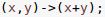
\includegraphics[width=0.3\linewidth]{image/double.png}
						\label{fig:double}
					\end{figure}
					\begin{figure}
						\centering
						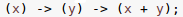
\includegraphics[width=0.4\linewidth]{image/curry.png}
						\label{fig:curry}
					\end{figure}
			\end{itemize}
	\end{itemize}
\end{frame}

%----------------------------------------------------------------------------------------

\begin{frame}
	\frametitle{\textbf{2.5 : Lambda calcolo vs Lambda Expressions}}
	\begin{itemize}
		\item
			\textbf{Booleani}:\\\
			\begin{itemize}
				\item 
					\textbf{Lambda calcolo}:\\\
						\[
							True = \lambda x.\lambda y.x
						\]
						\[
							False = \lambda x.\lambda y.y
						\]\\\
				\item 
					\textbf{Java}:\\\
					\begin{figure}
						\centering
						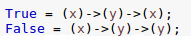
\includegraphics[width=0.4\linewidth]{image/booleani.png}
						\label{fig:identity}
					\end{figure}
			\end{itemize}	
	\end{itemize}
\end{frame}

%----------------------------------------------------------------------------------------

\begin{frame}
	\frametitle{\textbf{3 : Tipaggio Lambda Expression}}
	\begin{center}
		\textbf{\Huge Tipaggio Lambda Expression}
	\end{center}
\end{frame}

%----------------------------------------------------------------------------------------

\begin{frame}
	\frametitle{\textbf{3.1 : Tipaggio}}
	\begin{itemize}
		\item 
			Finora abbiamo trattato le \textit{Lambda Expression} senza specificare il modo in cui queste possono essere:\\\ 
			\begin{itemize}
				\item
					\textbf{Assegnate a una referenza};\\\
				\item
					\textbf{Passate come parametro};\\\
				\item
					\textbf{Ottenute come risultato di una valutazione}.\\\	
			\end{itemize}
			\textit{Entriamo nel dettaglio}
	\end{itemize}
\end{frame}

%----------------------------------------------------------------------------------------

\begin{frame}
	\frametitle{\textbf{3.1 : Tipaggio}}
	\begin{itemize}
		\item 
			Java è un linguaggio \textbf{strongly typed}, ciò significa che il programmatore è tenuto a specificare il tipo di ogni elemento che durante l'esecuzione denota un valore, e il linguaggio garantisce che tale valore sia utilizzato in modo coerente con il tipo specificato.\\\
		\item 
			Quindi, ogni sotto-espressione di qualsiasi espressione deve essere \textbf{ben tipata}.\\\
		\item 
			Tornando alle \textit{Lambda Expression}, il \textbf{tipo} di una \textit{Lambda Expression} deve essere coerente con il suo \textbf{Target Type}.
	\end{itemize}
\end{frame}

%----------------------------------------------------------------------------------------

\begin{frame}[fragile]
	\frametitle{\textbf{3.1 : Tipaggio}}
	\begin{itemize}
		\item 
			Per esempio, se scriviamo:\\\
			\begin{figure}
				\centering
				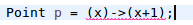
\includegraphics[width=0.3\linewidth]{image/target.png}
				\label{fig:target}
			\end{figure}
			Otteniamo il seguente errore:\\\
\begin{lstlisting}
	"The target type of this expression
	must be a functional interface"
\end{lstlisting}
		\item 
			Questo avviene, perchè la \textit{referenza} a una \textit{Lambda Expression} deve essere un' \textbf{Interfaccia Funzionale}.
	\end{itemize}
\end{frame}

%----------------------------------------------------------------------------------------

\begin{frame}
	\frametitle{\textbf{3.2 : Interfaccie funzionali}}
	\begin{itemize}
		\item
			Una qualunque \textit{interfaccia} è \textbf{funzionale} \textit{se e solo se}, contiene esattamente \textit{un solo} \textbf{metodo astratto}.\\\
		\item 
			La \textbf{signatura} di questo metodo, descrive il \textbf{TIPO} di una \textit{Lambda Expression}.\\\
		\item 
			Quindi il \textit{tipo} di una \textit{Lambda Expression} è un' \textbf{interfaccia funzionale}.\\\
		\item 
			Una \textit{Lambda Expression} è come se fosse un'\textit{istanza} di una classe concreta che implementa l'\textit{interfaccia funzionale}.
	\end{itemize}
\end{frame}

%----------------------------------------------------------------------------------------

\begin{frame}
	\frametitle{\textbf{3.2 : Interfaccie funzionali}}
	\begin{itemize}
		\item
			Adesso possiamo capire l'errore precedente:\\\
			\begin{figure}
				\centering
				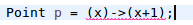
\includegraphics[width=0.3\linewidth]{image/target.png}
				\label{fig:target}
			\end{figure}
		\item
			In questo caso il \textit{type checker} da errore in quanto si aspetta che il \textit{target type} della \textit{Lambda Expression} sia di \textit{tipo Point}, quindi controlla che \textit{Lambda Expression} sia di \textit{tipo Point}, ma non può avere \textit{tipo Point} perchè \textit{Point} non è un'\textit{Interfaccia Funzionale}.
		\item
			Può avvenire che Point sia effettivamente un'interfaccia funzionale, ma la lambda potrebbe non matchare con la signatura del metodo astratto.
	\end{itemize}
\end{frame}

%----------------------------------------------------------------------------------------

\begin{frame}
	\frametitle{\textbf{3.3 : Typing}}
	\begin{itemize}
		\item
			Una \textit{Lambda Expression} può avere un \textit{tipo solo}, se questo è un'\textit{Interfaccia Funzionale}.\\\
		\item
			Il \textit{contesto} definisce il \textit{target type} che bisogna assegnare alla \textit{Lambda Expression}.\\\
		\item
			Il \textbf{target type} è :\\\
			\begin{itemize}
				\item
					Il \textit{tipo di ritorno} se il return di un metodo è una \textit{Lambda Expression};\\\
				\item
					Il \textit{tipo della variabile} se assegno alla variabile una \textit{Lambda Expression};\\\
				\item
					Il \textit{tipo del parametro} se passo una \textit{Lambda Expression} come parametro attuale;\\\
				\item
					Il \textit{tipo} a cui faccio \textit{cast} se la \textit{Lambda Expression} è un \textit{type-cast}.
			\end{itemize}
	\end{itemize}
\end{frame}

%----------------------------------------------------------------------------------------

\begin{frame}
	\frametitle{\textbf{3.3 : Typing}}
	\begin{itemize}
		\item
			A questo punto, il \textit{type-checker} considera il \textit{target-type} e controlla se può assegnarlo alla \textit{Lambda Expression}.\\\
			\begin{itemize}
				\item
					Se il \textit{target-type} non è un'\textit{Interfaccia Funzionale}, l'assegnazione viene subito \textbf{negata}.\\\
				\item
					Se il \textit{target-type} è un'\textit{Interfaccia Funzionale}, l'assegnazione avviene \textit{se e solo se}, la \textit{Lambda Expression} \textbf{matcha} la \textit{signatura} del metodo astratto, la quale è definita in questo modo :\\\
					\begin{center}
						\textbf{T metodo(T1 x)}\\\
					\end{center}
				\item
					Si controlla se assegnando alla variabile \textit{Lambda-astratta} il \textbf{tipo T1}, il \textit{body} della \textit{Lambda Expression} ha \textbf{tipo T}.
			\end{itemize}
	\end{itemize}
\end{frame}

%----------------------------------------------------------------------------------------

\begin{frame}
	\frametitle{\textbf{3.3 : Typing}}
	\begin{itemize}
		\item
			Java mette a disposizione le seguenti \textit{Interfacce Funzionali}, che possono essere usate per descrivere la \textit{signatura} di diverse \textit{Lambda Expression}:\\\
			\begin{itemize}
				\item
					\textbf{Predicate<T> \quad T $\rightarrow$ boolean}\\\
				\item
					\textbf{Function<T,R> \quad T $\rightarrow$ R}\\\
				\item
					\textbf{BinaryOperator<T> \quad (T,T) $\rightarrow$ T}\\\
				\item
					\textbf{BiFunction<T,U,R> \quad (T,U) $\rightarrow$ R}\\\
				\item
					\textbf{etc...}\\\
			\end{itemize}
		\item
			Inoltre Java, ti permette di definire nuove \textit{Interfacce Funzionali}, indicandole aggiungendo l'annotazione \textbf{@FunctionlInterface}.
	\end{itemize}
\end{frame}

%----------------------------------------------------------------------------------------

\begin{frame}[fragile]
	\frametitle{\textbf{3.3 : Typing}}
	\begin{itemize}
		\item
			\textit{Esempio} : \textbf{Function<T,R> \quad T $\rightarrow$ R}\\\
\begin{lstlisting}[language=Java]
 	public interface Function<T,R> {
		public R apply(T s);
	}
\end{lstlisting}
		\item 
			Quindi come fa il \textit{type checker} a stabilire se la seguente \textit{Lambda Expression} è \textit{ben tipata}?\\\
\begin{lstlisting}[language=Java]

Function<Integer,Boolean> fun = x->(x>=0);

\end{lstlisting}
	\end{itemize}
\end{frame}

%----------------------------------------------------------------------------------------

\begin{frame}[fragile]
	\frametitle{\textbf{3.3 : Typing}}
	\begin{itemize}
		\item
			\textbf{Controllo tipaggio}:\\\
			\begin{itemize}
				\item 
					Assunto il \textit{parametro x} di tipo Integer, il \textit{body} della \textit{Lambda Expression} è un Boolean.\\\
				\item 
					Dunque, assunto che $x$ è un intero, è vero che $x>=0$ è un booleano? Si, la \textit{Lambda Expression} è \textit{ben tipata}.
			\end{itemize}
	\end{itemize}
\end{frame}

%----------------------------------------------------------------------------------------

\begin{frame}[fragile]
	\frametitle{\textbf{3.3 : Typing}}
	\begin{itemize}
		\item
			E' possibile che il tipo di una \textit{Lambda Expression} sia compatibile con più \textit{target type}.\\\
\begin{lstlisting}[language=Java]

Predicate<Integer> p = (x)->(x%2==0);

Function<Integer, Boolean> f = (x)->(x%2==0);

\end{lstlisting}
	\end{itemize}
\end{frame}

%----------------------------------------------------------------------------------------

\begin{frame}[fragile]
\frametitle{\textbf{3.4 : Semantica}}
Supponiamo di aver definito la seguente interfaccia funzionale:
\begin{lstlisting}[language=Java]
interface I{
	boolean check(int n);
}
\end{lstlisting}
Supponiamo inoltre di avere anche definito una siffatta classe:
\begin{lstlisting}[language=Java]
class A<T> {
...
T method(I i){
	...
	int n;
	...
	i.check(n);
	...
}
}
\end{lstlisting}
\end{frame}

%----------------------------------------------------------------------------------------

\begin{frame}[fragile]
\frametitle{\textbf{3.4 : Semantica - Continuo:}}
Vediamo cosa avviene se in un client eseguo
\begin{lstlisting}[language=Java]
A<Integer> a = new A<>();
...
a.method((x)->(x>0));
\end{lstlisting}
Quando nel body del metodo incontro l'invocazione di check sulla lambda, viene eseguita l'istruzione
\begin{lstlisting}[language=Java]
return x>0;
\end{lstlisting}
Con il parametro formale x sostituito dal parametro attuale n (definito dal contesto del metodo).
\end{frame}

%----------------------------------------------------------------------------------------


\begin{frame}
	\frametitle{\textbf{4 : Lambda Expression vs Design Pattern}}
	\begin{center}
		\textbf{\Huge Lambda Expression\\ vs\\ Design Pattern}
	\end{center}
\end{frame}

%----------------------------------------------------------------------------------------

\begin{frame}[fragile]
	\frametitle{\textbf{4.1 : Perchè?}}
	\begin{itemize}
		\item
			Finora abbiamo visto alcune semplici applicazioni delle \textit{Lambda Expression}.\\\
		\item
			Adesso vediamo come viene \textbf{semplificato} il codice nel caso del loro utilizzo al posto dei \textit{Design Pattern}.\\\
		\item
			Qui di seguito faremo l'esempio dei seguenti \textit{Design Pattern}:\\\
			\begin{itemize}
				\item
					\textbf{Strategy};\\\
				\item
					\textbf{Template Method}.
			\end{itemize}
	\end{itemize}
\end{frame}

%----------------------------------------------------------------------------------------

\begin{frame}
	\frametitle{\textbf{4.2 : Strategy}}
	\begin{itemize}
		\item
			Il \textit{Design Pattern Strategy} con l'utilizzo delle \textit{Lambda Expression}, permette di scegliere fra funzioni diverse con la stessa signatura a run-time.\\\
		\item
			Esempio:\\\
			\begin{figure}
				\centering
				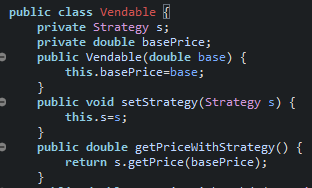
\includegraphics[width=0.5\linewidth]{image/strategy.png}
				\label{fig:target}
				\centering
				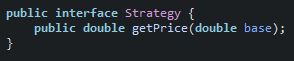
\includegraphics[width=0.4\linewidth]{image/interfaceStrategy.png}
				\label{fig:target}
			\end{figure}		
	\end{itemize}
\end{frame}

%----------------------------------------------------------------------------------------

\begin{frame}[fragile]
	\frametitle{\textbf{4.2 : Strategy}}
	\begin{itemize}
		\item
			Prima dell'introduzione delle \textit{Lambda Expression}, un client che avesse voluto implementare uno \textit{Strategy} avrebbe avuto due opzioni:\\\
			\begin{itemize}
				\item
					\textit{Classe anonima};\\\
				\item
					\textit{Definire una classe concreta che implementa l'interfaccia Strategy}.\\\
			\end{itemize}
		\item
			\textbf{Classe anonima}:\\\
			\begin{figure}
				\centering
				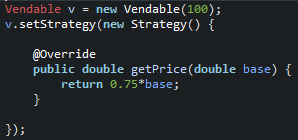
\includegraphics[width=0.6\linewidth]{image/strategyAnonima.png}
				\label{fig:target}
			\end{figure}
	\end{itemize}
\end{frame}

%----------------------------------------------------------------------------------------

\begin{frame}[fragile]
	\frametitle{\textbf{4.2 : Strategy}}
	\begin{itemize}
		\item
			\textbf{Definire una classe concreta che implementa l'interfaccia Strategy}:\\\
			\begin{figure}
				\centering
				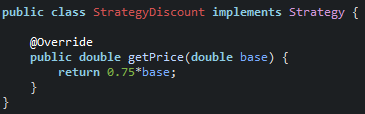
\includegraphics[width=0.6\linewidth]{image/strategyConcreta.png}
				\label{fig:target}
				\centering
				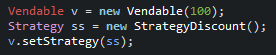
\includegraphics[width=0.6\linewidth]{image/createStrategy.png}
				\label{fig:target}
			\end{figure}
		\item
			\textbf{Lambda Expression}:\\\
			\begin{figure}
				\centering
				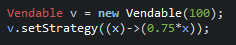
\includegraphics[width=0.6\linewidth]{image/lambdaStrategy.png}
				\label{fig:target}
			\end{figure}
	\end{itemize}
\end{frame}

%----------------------------------------------------------------------------------------

\begin{frame}
	\frametitle{\textbf{4.3 : Template Method}}
	\begin{itemize}
		\item
			Il \textit{Design Pattern Template Method} con l'utilizzo delle \textit{Lambda Expression}, permette di rimpiazzare il polimorfismo del metodo astratto con la composizione, passando una funzione al costruttore;\\\
		\item
			Esempio: \textbf{Polimorfismo del metodo astratto}				
			\begin{figure}
				\centering
				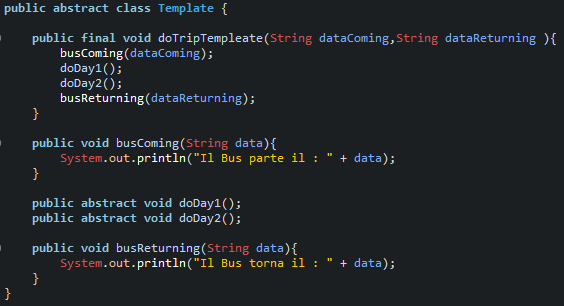
\includegraphics[width=0.8\linewidth]{image/template.png}
				\label{fig:target}
			\end{figure}
	\end{itemize}
\end{frame}

%----------------------------------------------------------------------------------------

\begin{frame}
	\frametitle{\textbf{4.3 : Template Method}}
	\begin{itemize}
		\item
			Prima dell'introduzione delle \textit{Lambda Expression}, un client che avesse voluto implementare un \textit{Template Method} avrebbe dovuto estendere in vari modi la classe concreta contenente il/i metodo/i astratto/i per differenziarlo/i:
			\begin{figure}
				\centering
				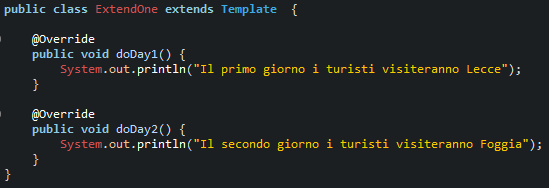
\includegraphics[width=0.7\linewidth]{image/extendOne.png}
				\label{fig:target}
				\centering
				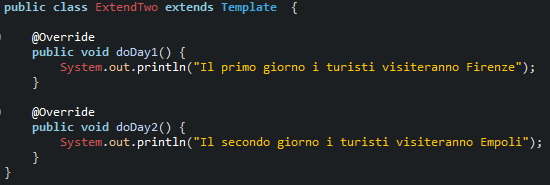
\includegraphics[width=0.7\linewidth]{image/extendTwo.png}
				\label{fig:target}
			\end{figure}
	\end{itemize}
\end{frame}

%----------------------------------------------------------------------------------------

\begin{frame}
	\frametitle{\textbf{4.3 : Template Method}}
	\begin{itemize}
		\item
			Nel metodo \textit{main()} avremo:
			\begin{figure}
				\centering
				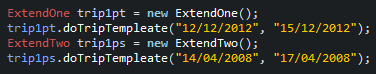
\includegraphics[width=0.6\linewidth]{image/mainTemplate.png}
				\label{fig:target}
			\end{figure}
		\item
			Ora implementiamo lo stesso programma con le \textbf{Lambda Expression}:
			\begin{figure}
				\centering
				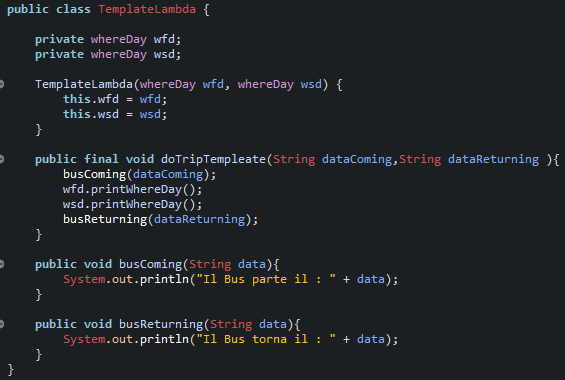
\includegraphics[width=0.6\linewidth]{image/templateLambda.png}
				\label{fig:target}
				\centering
				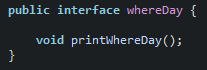
\includegraphics[width=0.3\linewidth]{image/interfaceTemplateLambda.png}
				\label{fig:target}
			\end{figure}
	\end{itemize}
\end{frame}

%----------------------------------------------------------------------------------------

\begin{frame}
	\frametitle{\textbf{4.3 : Template Method}}
	\begin{itemize}
		\item
			Nel metodo \textit{main()}, a questo punto avremo:
			\begin{figure}
				\centering
				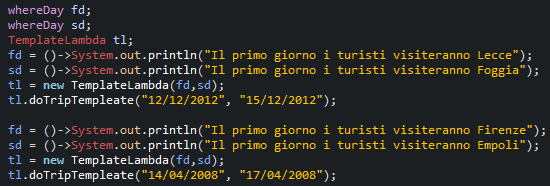
\includegraphics[width=0.9\linewidth]{image/mainTemplateLambda.png}
				\label{fig:target}
			\end{figure}
	\end{itemize}
\end{frame}

%----------------------------------------------------------------------------------------

\begin{frame}
	\frametitle{\textbf{4.4 : Altri Pattern}}
	\begin{itemize}
		\item
			Oltre a quelli appena descritti, si possono elencare tanti altri \textit{Design Pattern} e su come quest'ultimi possono essere implementati in modo diverso, possiamo dire \textit{migliore}, con l'utilizzo delle \textit{Lambda Expression}.\\\
		\item
			Tra i tanti, uno che sarebbe giusto nominare, è il \textit{Design Pattern Decorator}, che evitiamo di dimostrare.\\\
			\begin{itemize}
				\item
					Il \textit{Design Pattern Decorator} con l'utilizzo delle \textit{Lambda Expression}, permette di Passare una \textit{Lambda Expression} al metodo interessato, per \textit{modificarne il comportamento} (una \textit{Lambda Expression} che può chiamare un'altra \textit{Lambda Expression}, con la \textit{stessa signatura}, ma con \textit{argomenti diversi}).;
			\end{itemize}
	\end{itemize}
\end{frame}

%----------------------------------------------------------------------------------------

\begin{frame}
	\frametitle{\textbf{5 : Tipi Intersezione}}
	\begin{center}
		\textbf{\Huge Tipi Intersezione}
	\end{center}
\end{frame}

%----------------------------------------------------------------------------------------

\begin{frame}
	\frametitle{\textbf{5.1 : I tipi intersezione}}
	\begin{itemize}
		\item
			In Java 8 è stato introdotto un nuovo tipo.\\\
		\item
			I \textit{tipi intersezione}.
	\end{itemize}
\end{frame}

%----------------------------------------------------------------------------------------

\begin{frame}
	\frametitle{\textbf{5.2 : Regole dei tipi intersezione}}
		\begin{itemize}
		\item
			Se \textit{T, T'} sono tipi, allora \textit{T\&T'} è un tipo.\\\
		\item
			Un termine che ha tipo T e T', ha anche il tipo T\&T' .\\\
		\item
			Un termine che ha tipo T\&T', ha sia tipo T che tipo T', ossia ha tutte le proprietà del tipo T e le proprietà del tipo T'.\\\
		\item
			I tipi \textit{intersezione} sono particolarmente utili se usati assieme alle lambda, poichè castare una \textit{Lambda Expression} a un tipo \textit{interesezione} permette di aggiungere comportamenti diversi alla stessa \textit{Lambda Expression}.\\\
		\item
			Questo è l'argomento della successiva trattazione da parte della Prof.
	\end{itemize}
\end{frame}

%----------------------------------------------------------------------------------------

\begin{frame}
	\frametitle{\textbf{6 : Conclusioni}}
	\begin{center}
		\textbf{\Huge Conclusioni}
	\end{center}
\end{frame}

%----------------------------------------------------------------------------------------

\begin{frame}
	\frametitle{\textbf{6.1 : Conclusioni}}
	\begin{itemize}
		\item
			Abbiamo visto un'introduzione all'uso delle \textbf{Lambda Expression} in Java.\\\
		\item
			Java è un linguaggio nato per essere semplice, familiare e sicuro.\\\
		\item
			L'assenza delle \textit{Lambda Expression} rappresentava una grande lacuna rispetto ad altri linguaggi.\\\
		\item
			La loro aggiunta permette veramente di scrivere codice più conciso ed elegante.
	\end{itemize}
\end{frame}

%----------------------------------------------------------------------------------------

\begin{frame}
	\frametitle{\textbf{6.1 : Conclusioni}}
	\begin{itemize}
		\item
			Eliminata la necessità di dover implementare \textit{classi anonime} al volo.\\\
		\item
			Semplificazione di molti \textit{Design Pattern}.\\\
		\item
			Eliminazione di alcuni \textit{Design Pattern} (il Command può essere implementato con una \textit{Lambda Expression}).\\\
		\item
			L'utilizzo delle \textit{Lambda Expression} si combina bene con altri miglioramenti apportati al linguaggio:\\\
			\begin{itemize}
				\item 
					\textit{Referenza ai metodi statici};\\\
				\item
					\textit{Tipi intersezione}.
			\end{itemize}
	\end{itemize}
\end{frame}

%----------------------------------------------------------------------------------------

\end{document}
              